\section{Jerarqu\'ia de Memoria}
\begin{center}
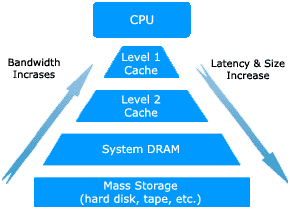
\includegraphics[scale=0.8]{./Graficos/jerarquia_memoria.png}
\end{center}

\vspace*{1\baselineskip}

El objetivo de esta jerarqu\'ia es aprovechar la referencia de \textit{localidad espacial} y la \textit{referencia de temporalidad}.

La primera  asume que si se accedi\'o a un dato, probablemente se vayan a acceder a datos contiguos; la segunda asume que un dato accedido
se va a volver a acceder pronto. Generalmente, la mayor\'ia de los accesos a un subsistema de memoria se hacen de manera transparente
entre un nivel de la jerarqu\'ia de memoria y el nivel inmediatamente superior o inferior. Por ejemplo, la CPU rara vez accede directamente
a la memoria principal, sino que cuando la CPU requiere datos de memoria, el subsistema de cache L1 se hace cargo. Si los datos requeridos
se encuentran en la cache L1, entonces \'esta entrega los datos a la CPU. En otro caso, el subsistema de cache L1 pasa el pedido al subsistema
de cache L2. Si los datos se encuentran en la cache L2, estos se pasan a la cache L1, y de la cache L1 a la CPU. Luego, si la CPU vuelve a solicitar
estos datos, los encontrar\'a en la cache L1.

Generalmente, los subsistemas de memoria mueven bloques de datos, o lineas de cache, cada vez que acceden a niveles inferiores de la jerarqu\'ia. Por 
ejemplo, si se ejecuta \textbf{mov eax, mem32}, y el valor de \textbf{mem32} no est\'a en la cache L1, el controlador de la cache no lee simplemente
los 32 bits de \textbf{mem32} de la cache L2, asumiendo que se encuentren ah\'i. En cambio, el controlador de la cache va a leer un bloque de bytes
 (16, 32 o 64) de la cache L2. Se espera que el programa exhiba localidad espacial y que por lo tanto los futuros accesos sean m\'as r\'apidos.
 

\section{Memoria Cache}

La memoria cache no se encuentra organizada como un conjunto de bytes, sino que se encuentra organizada en lineas de cache, donde cada linea contiene
16, 32 o 64 bytes.

Existen tres esquemas de cache diferentes: cache de mapeo directo, cache totalmente asociativa y cache asociativa en conjuntos de n v\'ias.

La memoria principal consiste de $2^{n}$ posiciones direccionables, con cada posici\'on teniendo una direcci\'on \'unica de $n$ bits. Para los
propositos del mapeo, se considera que esta memoria consiste de un conjunto de bloques de longitud fija de $k$ direcciones cada uno. Por lo tanto, hay
$M = \frac{2^{n}}{k}$ bloques en memoria principal, y la cache consiste en $m$ l\'ineas, cada una de las cuales contiene $k$ direcciones, m\'as unos
bits de tag y unos bits de control.

La cantidad de l\'ineas es considerablemente menor que la cantidad de bloques en memoria principal ($m << M$). Si una palabra en un bloque
de memoria principal es le\'ida, entonces todo el bloque es transferido a una de las l\'ineas de cache. Como varios bloques distintos pueden
ser copiados a una misma l\'inea, se incluye un tag que identifica qu\'e bloque en particular se encuentra actualmente en la l\'inea.

\subsection{Mapeo Directo}

\begin{center}
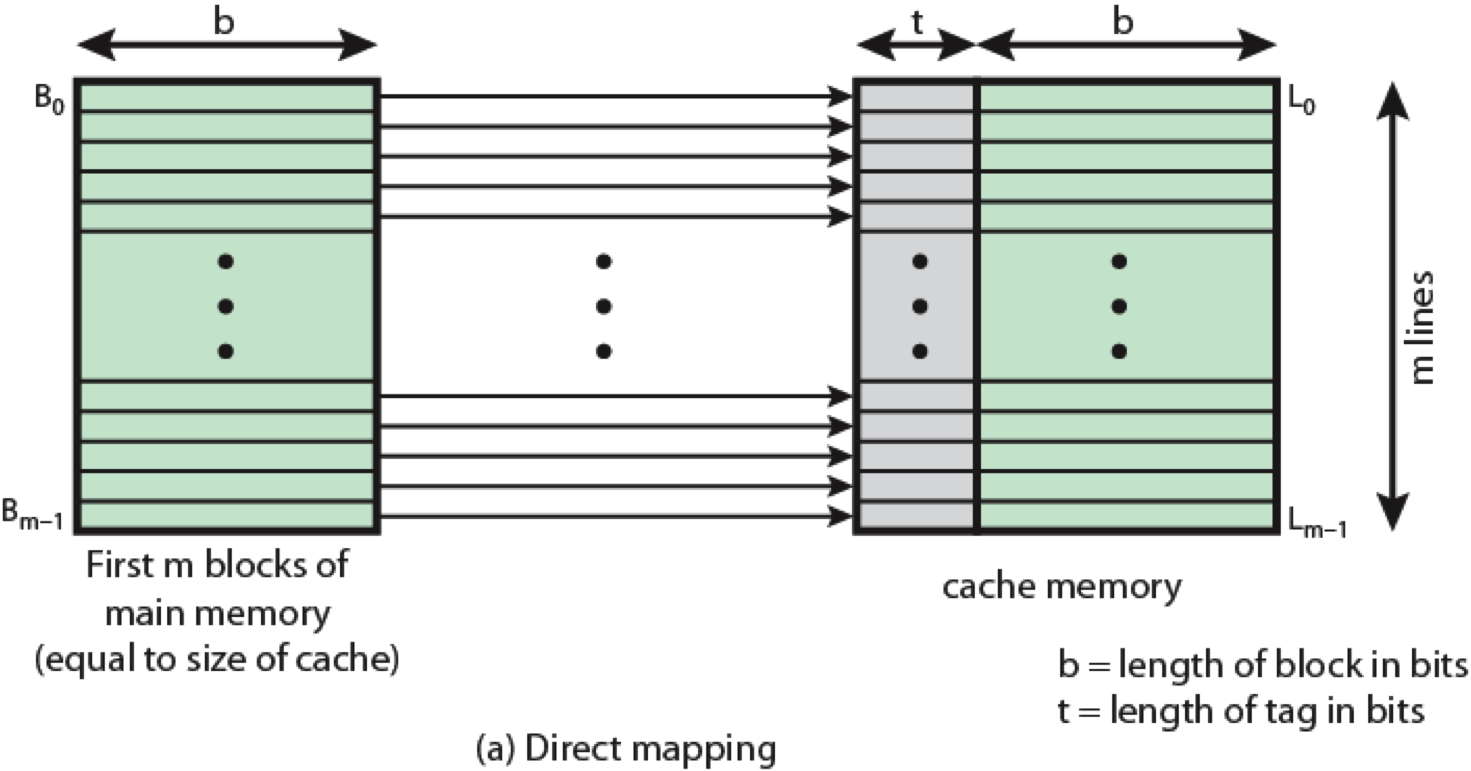
\includegraphics[scale=0.4]{./Graficos/mapeo_directo.png} 
\end{center}

En este esquema, cada bloque de memoria principal es mapeado a una \'unica posible l\'inea de cache. El mapeo se expresa como $i = j$ $mod$ $m$, donde

$i$ = n\'umero de la l\'inea de cache

$j$ = n\'umero de bloque de memoria principal

$m$ = cantidad de l\'ineas de la cache

Una desventaja de esto es que 2 bloques que mapean a la misma posici\'on se pueden estar continuamente pisando, sin usar el resto de la cache.


\subsection{Mapeo Totalmente Asociativo}

\begin{center}
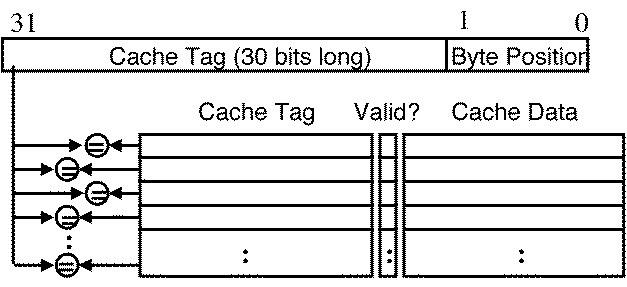
\includegraphics[scale=3.4]{./Graficos/totalmente_asociativa.png} 
\end{center}

El mapeo totalmente asociativo elimina la desventaja del mapeo directo permitiendo que un bloque de memoria principal sea cargado 
en cualquier l\'inea de la cache. Para determinar si un bloque se encuentra en la cache, la l\'ogica de control de la cache debe examinar 
simult\'aneamente el tag de todas las l\'ineas para encontrar un match. En este esquema hay cierta flexibilidad en cuanto a que bloque 
descartar cuando la cache est\'a llena y se lee un nuevo bloque.

La principal desventaja de este enfoque es la complejidad de los circuitos que se muestran para examinar todos los tags de la cache en paralelo.

Las direcciones de memoria se dividen de la siguiente manera:

\begin{center}
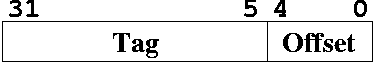
\includegraphics[scale=0.4]{./Graficos/totalmente_asociativa_2.png} 
\end{center}

\subsection{Mapeo Asociativo por Conjuntos}

En este caso, la cache consiste en un n\'umero de conjuntos, cada uno de los cuales consiste en un n\'umero de l\'ineas. Las 
relaciones son: 

$m = $ $v*k$ 

$i =$ $j$ $mod$ $k$

donde

$i =$ n\'umero del conjunto

$j =$ n\'umero del bloque de memoria principal

$m =$ cantidad de l\'ineas en la cache

$v =$ cantidad de conjuntos

$k =$ cantidad de l\'ineas en cada conjunto

Esto se denomina cache asociativa por conjuntos de k-v\'ias. En el mapeo asociativo por conjuntos, cada palabra se puede mapear
a cualquier l\'inea de cache en un conjunto espec\'ifico. Por lo tanto, la cache asociativa por conjuntos se puede implementar 
f\'isicamente como $v$ caches asociativas. 


\begin{center}
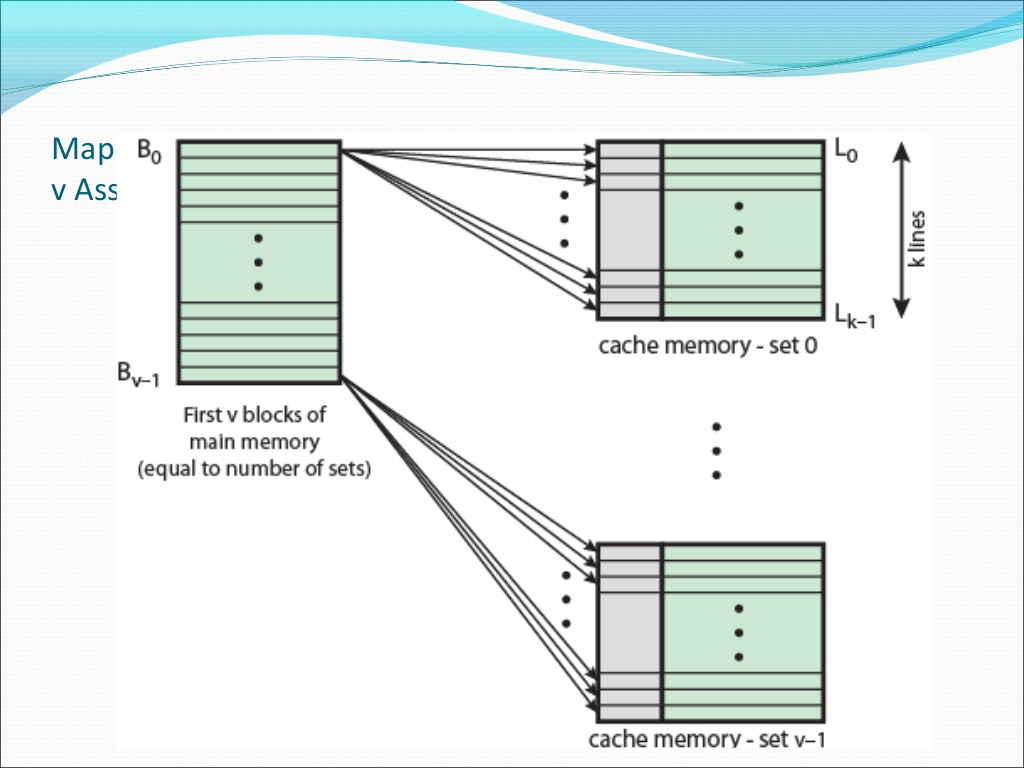
\includegraphics[scale=0.3]{./Graficos/asociativa_por_conjuntos.jpg} 
\end{center}

Tambi\'en se pueden implementar como $k$ caches de mapeo directo. Cada cache de mapeo directo se la denomina una v\'ia, que consiste
en $v$ l\'ineas. Las primeras $v$ l\'ineas de memoria principal se mapean directamente en las $v$ l\'ineas de la v\'ia, y as\'i sucesivamente.


\begin{center}
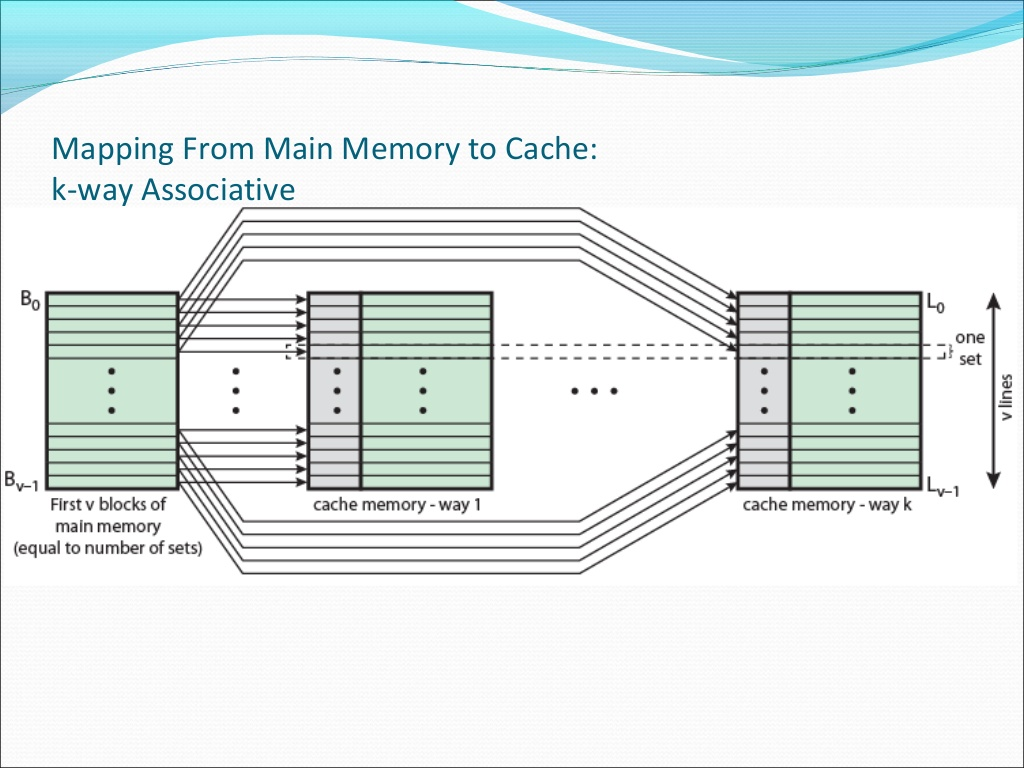
\includegraphics[scale=0.3]{./Graficos/asociativa_por_conjuntos_2.jpg} 
\end{center}

En este caso, la controladora de la cache interpreta las direcciones de memoria como 3 campos: Tag, Set y Offset.


\begin{center}
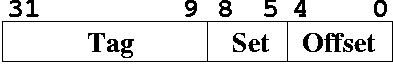
\includegraphics[scale=0.5]{./Graficos/asociativa_por_conjuntos_3.png} 
\end{center}

\newpage
\subsection{Algoritmos de Reemplazo}

Una vez que la cache est\'a llena, si se trae un nuevo bloque a la cache, se debe descartar uno de los bloques existentes. Para hacer esto,
se debe implementar un algoritmo en hardware. Uno de los m\'as efectivos es LRU (least recently used): reemplazar en la cache el bloque
que hace m\'as tiempo que no es usado. Otra posibilidad es usar un algoritmo FIFO, y reemplazar el bloque que hace m\'as tiempo que
est\'a en la cache. Por \'ultimo, se puede utilizar un algoritmo de LFU (least frequently used), que reemplaza el bloque que experiment\'o
la menor cantidad de referencias.

\subsection{Pol\'iticas de Escritura}

Cuando un bloque de la cache es reemplazado, existen 2 casos a considerar: si el bloque viejo no fue alterado, entonces puede ser reemplazado
sin m\'as; en otro caso, la memoria principal debe ser actualizada antes de descartar el bloque. Existen dos problemas con respecto a esto. 
Primero, m\'as de un dispositivo puede tener acceso a la memoria principal, por ejemplo un dispositivo de E/S. Si una palabra ha sido alterada
en la cache, entonces la palabra correspondiente en memoria es inv\'alida, y si el dispositivo de E/S alter\'o una palabra en la memoria
principal, entonces esa palabra en la cache es inv\'alida.

Otro problema que ocurre es cuando se tienen varios procesadores compartiendo el mismo bus y cada uno tiene su propia cache. Entonces, si una
palabra es alterada en una cache, puede invalidar el resto de las caches.

La t\'ecnica m\'as simple es el \textbf{write through}. Con esta t\'ecnica, todas las operaciones de escritura son hechas a la memoria principal
y a la cache, asegurando que la memoria principal siempre es v\'alida. La desventaja principal de esta t\'ecnica es que genera mucho
tr\'afico de memoria, lo cual puede ocasionar un bottleneck. Con \textbf{write through buffered}, el procesador actualiza la cache, y el controlador
cache luego actualiza la copia en memoria DRAM mientras el procesador contin\'ua ejecutando instrucciones y usando datos de la memoria cache.

Otra t\'ecnica, conocida como \textbf{write back}, minimiza las escrituras a memoria, ya que las actualizaciones se hacen solo en la cache. Cuando
se hace una actualizaci\'on, se prende un bit asociado con la l\'inea de cache llamado dirty bit. Entonces, cuando un bloque es reemplazado, 
es escrito en memoria principal si y solo si el bit dirty est\'a encendido. El problema con esta pol\'itica es que porciones de la memoria principal
pueden ser inv\'alidas, y por lo tanto accesos de dispositivos de E/S solo se pueden realizar a traves de la cache, lo cual puede crear un bottleneck.

\newpage
\section{Direccionamiento de Memoria}

En los procesadores 80x86 existen 3 tipos distintos de direcciones.

\begin{itemize}
 \item \underline{Direcciones l\'ogicas:} est\'an relacionadas con la arquitectura de segmentos de los 80x86. Cada direcci\'on l\'ogica consiste
 en un segmento y en un offset, que denota la distancia desde el inicio del segmento hasta la direcci\'on buscada.
 \item \underline{Direcciones lineales (o virtuales):} un entero sin signo de 32 bits que puede direccionar hasta 4GB.
 \item \underline{Direcciones f\'isicas:} son las direcciones f\'isicas de la memoria.
\end{itemize}

\begin{center}
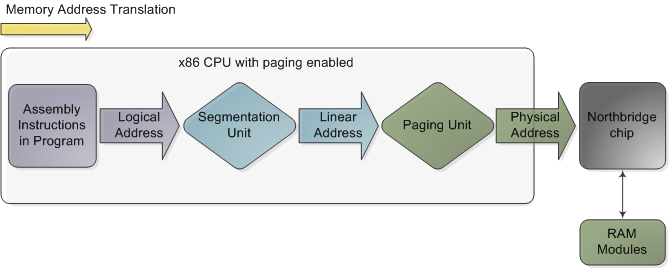
\includegraphics[scale=0.5]{./Graficos/direccionamiento_memoria.png} 
\end{center}

\subsection{Segmentaci\'on en Hardware}

\subsubsection{Selectores de segmento y registros de segmentaci\'on}

Una direcci\'on l\'ogica consiste de dos partes: un identificador de segmento y un offset que especifica la direcci\'on relativa 
dentro del segmento. El identificador de segmento es un campo de 16 bits llamado \textbf{selector de segmento}, mientras que el offset
es un campo de 32 bits.

El procesador provee \textbf{registros de segmentaci\'on} cuyo \'unico prop\'osito es guardar los selectores de segmento. Los registros son:
\textit{cs, ss, ds} de prop\'osito espec\'ifico, y \textit{es, fs, gs} de prop\'osito general. El registro \textit{cs} tiene otra funci\'on
importante: incluye un campo de 2 bits que especifica el \textit{Request Privilege Level} (RPL) de la CPU.

\begin{center}
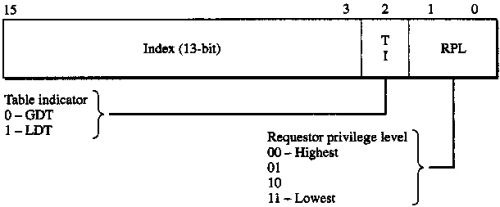
\includegraphics[scale=0.5]{./Graficos/selector_segmento.png} 
\end{center}

El \'indice identifica la entrada del descriptor de segmento en la GDT o LDT. Como los descriptores de segmento son de 8 bytes, el \'indice se
debe multiplicar por 8.

El TI (Table Indicator) especifica si el descriptor de segmento est\'a en la GDT (TI = 0) o en la LDT (TI = 1).

El RPL especifica el CPL de la CPU cuando el selector de segmento es cargado en el registro cs.

Como Linux pr\'acticamente no utiliza segmentaci\'on salvo donde lo requiera el procesador, el offset de una direcci\'on l\'ogica coincide
siempre con la direcci\'on lineal.

\subsubsection{Descriptores de Segmento}

Cada segmento est\'a representado por un \textbf{descriptor de segmento} de 8 bytes, el cual est\'a guardado en la \textit{Global Descriptor Table}
(GDT) o en la \textit{Local Descriptor Table} (LDT).

Existen varios tipos de descriptores de segmento:

\begin{itemize}
 \item \underline{Descriptor de segmento de c\'odigo:} indica que el descriptor de segmento se refiere a un segmento de c\'odigo. Puede
 estar en la GDT o en la LDT.
 \item \underline{Descriptor de segmento de datos:} indica que el descriptor de segmento se refiere a un segmento de datos. Puede estar en la 
 GDT o en la LDT. Un segmento de stack se implementa mediante un segmento de datos gen\'erico.
 \item \underline{Descriptor de segmento de estado de tarea:} indica que el descriptor de segmento se refiere a un Task State Segment (TSS), es decir, un
 segmento usado para guardar los contenidos de los registros del procesador. Puede estar solo en la GDT.
\end{itemize}

Cada vez que un selector de segmento se carga en un registro de segmento, el correspondiente descriptor de segmento es cargado en un registro
especial que no es accesible al programador. De esta manera, las traducciones de direcciones l\'ogicas referidas a ese segmento se pueden realizar sin pasar
por la GDT. Este registro se actualiza cada vez que cambia el selector de segmento.


\subsubsection{Paginaci\'on en Hardware}

La unidad de paginaci\'on traduce las direcciones lineales en direcciones f\'isicas. Una funci\'on fundamental de la unidad es chequear el tipo
de acceso requerido contra los derechos de acceso de la direcci\'on lineal; si el acceso a memoria no es v\'alido, genera un Page Fault.

Por una cuesti\'on de eficiencia, las direcciones lineales est\'an agrupadas en intervalos de longitud fija llamados p\'aginas; direcciones lineales
continuas dentro de una p\'agina est\'an mapeadas en direcciones f\'isicas continuas.

De esta manera, el kernel puede especificar la direcci\'on f\'isica y los derechos de acceso de una p\'agina en vez de los de las direcciones lineales
inclu\'idas en ella.

Las estructuras de datos que mapean direcciones lineales a f\'isicas son llamadas page tables. Est\'an guardadas en memoria principal y deben ser
inicializadas antes de habilitar la paginaci\'on.

\subsubsection{Paginaci\'on Regular}

La traducci\'on de la direcci\'on lineal se realiza en 2 pasos, cada uno basado en una tabla de traducci\'on. El objetivo de este esquema en dos
niveles es reducir la cantidad de memoria RAM necesaria para las page tables de cada proceso. Si se utilizase un solo nivel de tablas, se
necesitar\'ian $2^{20}$ entradas (4 bytes por entrada = 4 MB) para representar las page tables de cada proceso. El esquema con 2 niveles reduce la
cantidad de memoria necesaria ya que requiere page tables solo para aquellas regiones de memoria virtual realmente usadas por el proceso.


\begin{center}
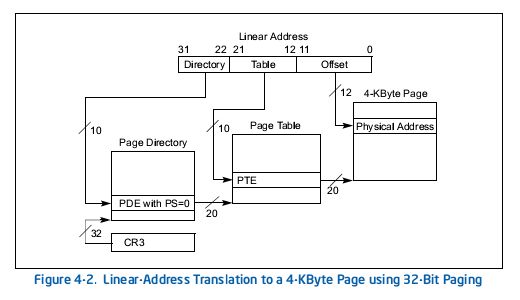
\includegraphics[scale=0.6]{./Graficos/linear_address_translation.png} 
\end{center}

\newpage
\subsubsection{Paginaci\'on Extendida}

En la paginaci\'on extendida, las p\'aginas son de 4 MB en vez de 4 KB.

\begin{center}
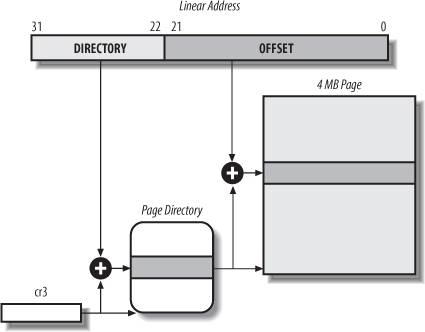
\includegraphics[scale=0.6]{./Graficos/extended_paging.jpg} 
\end{center}


\subsubsection{Physical Address Extension (PAE)}

La cantidad de memoria RAM que soporta un procesador est\'a limitada por el n\'umero de pins de direcciones conectados al bus de direcciones. Los
procesadores del 80386 hasta el Pentium direccionan hasta 4 GB de memoria.

Como algunas computadoras necesitaban m\'as memoria (dentro de la arquitectura 80x86 de 32 bits), Intel aument\'o el n\'umero de los pins de direcciones
de 32 a 36. Esto puede ser explotado con un nuevo sistema de paginaci\'on que permita traducir direcciones lineales de 32 bits en direcciones f\'isicas de 36 bits.


\newpage

\section{Modos de Operaci\'on}

Los procesadores IA-32 tienen 3 modos de operaci\'on:


\begin{itemize}
 \item \underline{Modo Real:} en este modo el procesador implementa el entorno de operaci\'on del 8086 con algunas extensiones: puede pasar por
 software a Modo Protegido o a Modo Mantenimiento del Sistema y utilizar registros de 32 bits.
 \item \underline{Modo Protegido:} en este modo se implementa multitasking y se despliega un espacio de direccionamiento de 4 GB, extensible a
 64 GB. A partir del 80386 se introduce un sub modo al que puede ponerse a una determinada tarea, denominado Virtual-8086, que permite a un programa
 dise\~nado para ejecutarse en 8086, poder ejecutarse como una tarea en Modo Protegido.
 \item \underline{Modo Mantenimiento del Sistema:} este modo fue introducido para realizar funciones espec\'ificas para la plataforma de hardware en la
 cual se desempe\~na el procesador, como ahorro de energ\'ia y seguridad.
\end{itemize}

Los procesadores Intel 64 adem\'as de los modos de trabajo de los IA-32 incluyen un modo IA-32e, al que se pasa estando en Modo Protegido, con paginaci\'on
habilitada y PAE activo. En este modo existen a su vez 2 sub modos: Compatibilidad y Modo 64 bits.

\begin{itemize}
 \item \underline{Modo Compatibilidad:} este modo permite a las aplicaciones de 16 y 32 bits ejecutarse sin recompilaci\'on bajo un sistema operativo
 de 64 bits. El entorno de ejecuci\'on es el de la arquitectura IA-32, y no soporta el manejo de tareas del modo IA-32 (TSS mediante) ni el modo Virtual-8086.
 \item \underline{Modo 64 bits:} este modo habilita al sistema operativo de 64 bits a ejecutar tareas utilizando direcciones lineales de 64 bits.
\end{itemize}

\newpage

\section{Taxonom\'ia de Flynn}

Es la manera m\'as com\'un de categorizar a los sistemas con capacidad de procesamiento paralelo.

\begin{itemize}
 \item \underline{Single Instruction, Single Data (SISD):} un solo procesador ejecuta un solo flujo de instruccione que operan en datos almacenados en una sola memoria.
 \item \underline{Single Instruction, Multiple Data (SIMD):} una sola instrucci\'on de m\'aquina controla la ejecuci\'on simult\'anea de un n\'umero de elementos.
 \item \underline{Multiple Instruction, Single Data (MISD):} no existen muchas arquitecturas que lo implementen.
 \item \underline{Multiple Instruction, Multiple Data (MIMD):} CLusters, SMP, NUMA.
\end{itemize}

\newpage

\section{Symmetric Multiprocessors (SMP)}

Un SMP puede definirse como un sistema con las siguientes caracter\'isticas:

\begin{itemize}
 \item Hay 2 o m\'as procesadores de capacidad similar.
 \item Estos procesadores comparten la misma memoria principal y dispositivos de E/S, y est\'an interconectados por un bus, de manera tal que
 el tiempo de acceso a la memoria es aproximadamente el mismo para cada procesador.
 \item Todos los procesadores pueden realizar las mismas operaciones (de ah\'i sim\'etrico).
 \item Un sistema operativo que provea interacci\'on entre los procesadores y las tareas
\end{itemize}

Cada procesador tiene acceso a la memoria principal y a los dispositivos de E/S a traves de alg\'un mecanismo de intercomunicaci\'on. Los procesadores
se pueden comunicar entre s\'i mediante memoria o intercambiando se\~nales directamente.

La organizaci\'on m\'as com\'un es la del bus de tiempo compartido. La estructura y las interfaces son b\'asicamente las mismas que para un sistema
de un solo procesador. El bus consiste en lineas de control, direcciones y datos. La desventaja principal es la performance, ya que como todas las referencias
a memoria pasan a traves de un bus com\'un, la velocidad del bus limita la velocidad de todo el sistema.

Para mejorar la performance, cada procesador cuenta con una memoria cache interna. Esto introduce nuevos problemas, ya que si un dato es modificado en una cache, puede
invalidar al mismo dato en otra cache.

Este problema es conocido como el problema de la coherencia de cache, y la soluci\'on t\'ipicamente involucra cambios de hardware.

\subsection{Coherencia de Cache}

En los sistemas nultiprocesador, es com\'un que cada procesador tenga varios niveles de cache, aunque esto crea un problema llamado ``coherencia
de cache''. La esencia del problema es esta: m\'ultiples copias del mismo dato pueden existir en diferentes caches simult\'aneamente, y si cada
procesador actualiza su copia, se tiene una visi\'on inconsistente de la memoria. Dos pol\'iticas comunes de escritura en caches son:

\begin{itemize}
 \item \underline{Write Back:} las operaciones de escritura se hacen solo a la cache. La memoria principal se actualiza cuando la l\'inea de cache se
 remueve de la cache.
 \item \underline{Write Through:} todas las operaciones de escritura se realizan tanto en la cache como en la memoria principal.
\end{itemize}

Es claro que la pol\'itica de Write Back puede resultar en una inconsistencia. Si 2 caches contienen la misma linea, y la linea se actualiza
en una cache, la otra cache contendr\'a un valor inv\'alido. Incluso con la pol\'itica de Write Through pueden ocurrir inconsistencias a menos
que las otras caches reciban una notificaci\'on de la actualizaci\'on.

\subsubsection{Soluciones por Software}

Los esquemas de coherencia de cache por software dependen del compilador y el sistema operativo para tratar con el problema.

La ventaja de este enfoque es que transfiere el overhead de detectar potenciales problemas de tiempo de ejecuci\'on a tiempo de compilaci\'on, y
la complejidad de dise\~no del hardware al software. La desventaja es que el software muchas veces debe tomar decisiones conservadoras, lo cual
lleva a una utilizaci\'on ineficiente de la cache. Una posible pol\'itica es marcar algunos datos como no cacheables.

\subsubsection{Soluciones por Hardware}

Las soluciones basadas en hardware son generalmente referidas como protocolos de coherencia de cache. Estas soluciones proveen reconocimiento
en tiempo de ejecuci\'on de potenciales inconsistencias. Como el problema solamente es tratado cuando realmente aparece, hay un uso m\'as efectivo
de la cache, llevando a una mejora en performance con respectoa a enfoques basados en software. Adem\'as, estos enfoques son transparentes al programador.

En los esquemas de hardware existen 2 categor\'ias:

\begin{itemize}
 \item \underline{Protocolos de Directorio:} los protocolos de directorio recolectan y mantienen informaci\'on sobre donde residen las copias de las lineas.
 Generalmente, hay un controlador centralizado que es parte del controlador de la memoria principal, y un directorio que est\'a almacenado en memoria principal.
 
 El directorio contiene informaci\'on de estado global sobre los contenidos de las caches. Cuando un controlador individual de cache hace un pedido, 
 el controlador centralizado chequea y env\'ia los comandos necesarios para tranferir datos entre memoria y cache o entre caches. Tambi\'en es responsable de mantener
 la informaci\'on de estado actualizada.
 
 Generalmente, el controlador mantiene informaci\'on acerca de qu\'e procesadores tienen una copia de qu\'e l\'ineas. Antes de que un procesador pueda escribir
 a una copia local de la l\'inea, debe pedir acceso exclusivo a esa l\'inea al controlador. Antes de otorgar acceso exclusivo, el controlador manda un mensaje
 a todos los procesadores con una copia en la cache de esta l\'inea para que la invaliden.
 
 La desventaja de este esquema es que existe un cuello de botella entre los controladores de cache y el controlador central.
 
 \item \underline{Protocolos Snoop:} estos protocolos distribuyen la responsabilidad de mantener la coherencia de cache entre todos los controladores
 de cache del sistema. Una cache debe reconocer cuando una linea que posee es compartida con otras caches. Cuando se actualiza una linea, se 
 anuncia esto a todas las demas caches mediante un mecanismo de broadcasting. Cada controladora de cache puede ``hurgar'' (snoop) en la red para
 observar estas notificaciones y actuar en consecuencia.
 
 Se han explorado dos enfoques: \textbf{Write Invalidate} y \textbf{Write Update}. Con un protocolo Write invalidate, pueden haber varios lectores
 pero un solo escritor en un momento dado. Cuando una cache quiere realizar una escritura, primero env\'ia un mensaje que invalida esa l\'inea en las demas
 caches, haciendo que la l\'inea sea exclusiva para la cache de escritura.
 
 Con el protocolo Write Update, pueden haber m\'ultiples escritores y lectores. Cuando un procesador quiere actualizar una l\'inea compartida, la palabra
 a ser actualizada es distribu\'ida a los dem\'as procesadores.
 
 El protocolo Write Invalidate marca el estado de cada l\'inea de cache (usando 2 bits del tag) como modificado, exclusivo, compartido (shared) e inv\'alido.
 Por esta raz\'on, a este protocolo se lo llama \textbf{protocolo MESI}.
\end{itemize}

\subsection{Protocolo MESI}

Para este protocolo, la cache de datos incluye 2 bits de status por cada tag, por lo que cada l\'inea puede estar en uno de cuatro estados:

\begin{itemize}
 \item \underline{Modificado:} la l\'inea en la cache ha sido modificada y est\'a disponible solo en esa cache, y es diferente al dato que est\'a en memoria principal.
 \item \underline{Exclusivo:} la l\'inea en la cache es la misma que la que est\'a en memoria principal y no est\'a presente en otras caches.
 \item \underline{Shared:} la l\'inea en la cache es la misma que la que est\'a en memoria principal y puede estar presente en otra cache.
 \item \underline{Inv\'alido:} la l\'inea en la cache contiene datos inv\'alidos.
\end{itemize}

\begin{center}
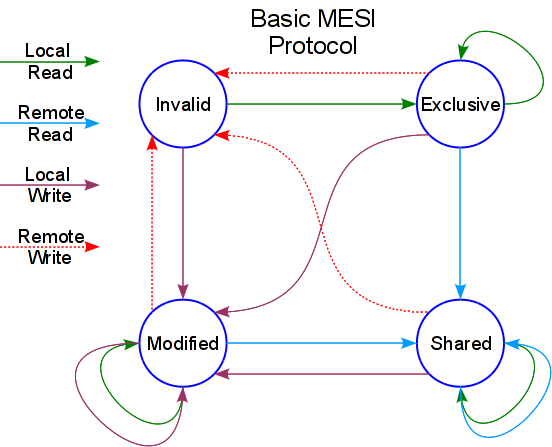
\includegraphics[scale=0.6]{./Graficos/MESI.png} 
\end{center}


\section{Instruction Pipelining}

Es una t\'ecnica utilizada para aumentar el throughput de instrucciones (cantidad de instrucciones ejecutadas por unidad de tiempo). El ciclo
de instrucciones se parte en series llamadas pipelines, y cada uno de estos pasos puede ser ejecutado concurrentemente.

El pipelining incrementa el throughput de instrucciones al hacer m\'ultiples operaciones concurrentemente, pero no reduce la latencia de las instrucciones
(el tiempo que tardan en completarse). De hecho, puede aumentar la latencia debido al overhead de dividir las instrucciones, o debido a que el pipeline
debe pararse.

El objetivo es que el procesador trabaje con tantas instrucciones a la vez como pasos independientes hay en una instrucci\'on.

Hay ciertos factores que limitan la performance; por ejemplo, si la duraci\'on de las etapas no es igual, otras partes del pipeline van a 
tener que quedarse en espera. Otra dificultad es el branching condicional de las instrucciones, que puede invalidar muchas instrucciones
levantadas. Otro evento impredecible es una interrupci\'on.

En principio parece que mientras mayor n\'umero de etapas haya en un pipeline, mayor es el ritmo de ejecuci\'on. Sin embargo, esto no es as\'i por
2 motivos:

\begin{itemize}
 \item En cada etapa del pipeline hay cierto overhead en mover los datos entre los distintos buffers. Esto es significativo cuando las instrucciones
 secuenciales son l\'ogicamente dependientes, ya sea por el uso de branching o por el acceso a memoria.
 \item La cantidad de l\'ogica de control requerida para manejar dependencias de memoria y registros y para optimizar el uso del pipeline aumenta
 enormemente con el n\'umero de etapas.
\end{itemize}


\begin{center}
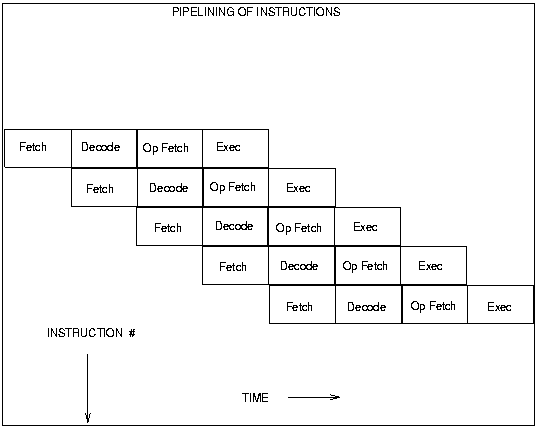
\includegraphics[scale=0.4]{./Graficos/pipeline.png} 
\end{center}


\subsection{Branches}

Uno de los mayores problemas al dise\~nar un pipeline es asegurarse que continuamente lleguen instrucciones a las etapas iniciales. El principal
impedimento para esto es el branching condicional, y existen varios enfoques para tratarlo:

\begin{itemize}
 \item \underline{Flujos M\'ultiples:} consiste en replicar las porciones iniciales del pipeline y levantar instrucciones de ambos branches
 \item \underline{Loop Buffer:} consiste en una peque\~na memoria muy r\'apida, que es mantenida por la etapa del fetch de instrucciones del 
 pipeline, y contiene las $n$ instrucciones secuenciales m\'as recientemente levantadas. Si se tiene que tomar un branch, el hardware chequea si
 el branch est\'a en el buffer; si es as\'i, la pr\'oxima instrucci\'on se levanta del buffer.
 \item \underline{Branch Prediction:} existen varias t\'ecnicas para predecir si se va a tomar cierto branch. Algunas de las m\'as comunes son:
 \begin{itemize}
  \item Predict Never Taken
  \item Predict Always Taken
  \item Predict by Opcode
  \item Taken/not Taken switch
  \item Branch History Table
 \end{itemize}
\end{itemize}

Los tres primeros enfoques son est\'aticos: no dependen de la ejecuci\'on del programa al momento de ejecutar la instrucci\'on condicional.

En Predict Never Taken, el procesador asume por default que el salto nunca se toma, es decir que contin\'ua levantando las instrucciones siguientes
a las del salto. Funciona bien cuando el salto es ``hacia adelante''.

En Predict Always Taken, el procesador asume que el salto se toma siempre, es decir levanta las instrucciones a partir de la direcci\'on target.

En Predict by Opcode, el procesador asume que el branch va a ser tomado para ciertos opcodes de branch y no para otros.

En los enfoque din\'amicos, la idea es aumentar la cantidad de aciertos guardando informaci\'on sobre las instrucciones de branch condicional, 
por ejemplo con 1 o m\'as bits. Estos bits son referidos como taken/not taken switchs que hacen que el procesador tome una decisi\'on particular
la pr\'oxima vez que encuentre la instrucci\'on.

Con 1 solo bit, todo lo que se puede registrar es si la \'ultima ejecuci\'on de la instrucci\'on result\'o en un branch o no. Una limitaci\'on
que tiene es que si un salto siempre resulta taken y falla una vez, produce dos predicciones fallidas seguidas, ya que el bit se invierte.

Para superar esta limitaci\'on, se utilizan 2 bits, generando un proceso de decisi\'on que se puede representar como una m\'aquina de estados finitos
con 4 estados

\begin{center}
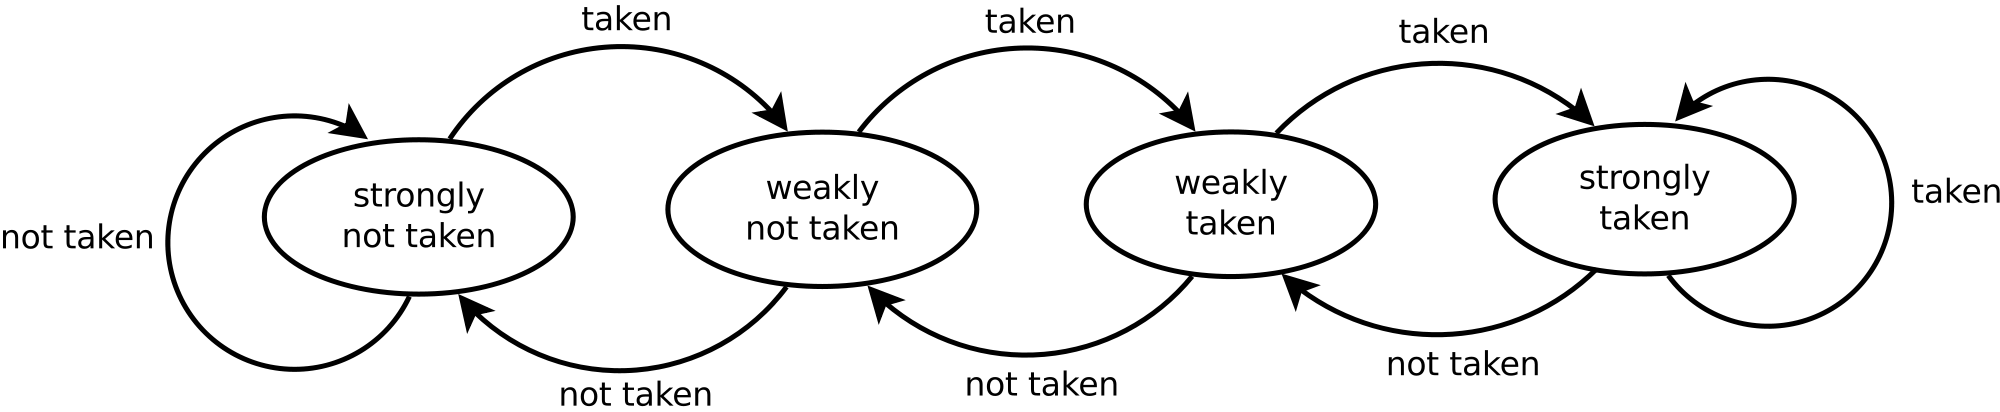
\includegraphics[scale=0.2]{./Graficos/branch_prediction.png} 
\end{center}


En la pr\'actica este tipo de branch prediction se implementa en la etapa de instruction fetch del pipeline, como un peque\~no cache de 
direcciones. Otra forma de implementarlo es agregar un par de bits a cada bloque de lineas en el cache de instrucciones, que se emplean
\'unicamente si ese bloque tiene instrucciones de salto condicional.

\subsection{Hazards}

En pipelining hay situaciones donde la siguiente instrucci\'on no se puede ejecutar en el siguiente ciclo. Estas situaciones se llaman hazards, y existen
3 tipos:

\begin{itemize}
 \item \underline{Hazard estructural:} ocurre cuando el hardware no soporta la combinaci\'on de instrucciones que queremos ejecutar en un mismo ciclo de reloj.
 Ej: accesos concurrentes a memoria.
 \item \underline{Hazard de datos:} ocurre cuando se para el pipeline debido a que una etapa debe esperar a que otra termine. Por ejemplo, si se hace
 una suma que se guarda en un registro, y luego se utiliza ese registro para hacer una resta. Para mitigar este problema se utiliza una 
 t\'ecnica llamada forwarding, que consiste en extraer el resultado directamente de la salida de la unidad de ejecuci\'on y enviarlo a la entrada
 de la etapa que lo requiere.
 \item \underline{Hazard de control:} ocurre cuando se tiene que tomar una decisi\'on basada en el resultado de una instrucci\'on mientras
 otras se est\'an ejecutando.
\end{itemize}


\newpage

\section{Procesadores Superescalares}

Un procesador superescalar es un procesador que utiliza m\'ultiples pipelines independientes para ejecutar las instrucciones. Estos procesadores
explotan lo que se llama paralelismo a nivel de instrucci\'on, que se refiere al grado en que las instrucciones de un programa se pueden 
ejecutar en paralelo.

Otro enfoque para mejorar la performance es el \textbf{superpipelining}, en donde las etapas del pipeline se dividen en etapas m\'as peque\~nas, y al
hacer cada etapa menos trabajo, se puede aumentar la velocidad del clock.

Estos procesadores tienen desventajas similares a las que surgen con pipelining:

\begin{itemize}
 \item \underline{Data Hazards:} se da en situaciones como la siguiente:\\
 \textit{add r1, r2}\\
 \textit{add r3, r1}
 
 La segunda instrucci\'on se puede levantar y decodificar pero no se puede ejecutar hasta que termine la primera instrucci\'on. Para
 mitigar esto se utilizan t\'ecnicas como register renaming y out of order execution.
 
 \item \underline{Structural Hazards:} se da cuando el procesador no tiene suficientes recursos para ejecutar varias instrucciones a la vez.
 Por ejemplo: \\
 \textit{add r1, r2}\\
 \textit{add r3, r4}\\
 El procesador debe tener la capacidad de realizar 2 writes a la vez.
 
 \item \underline{Control Hazards:} se dan cuando el procesador llega a un branch, y tiene que decidir qu\'e instrucci\'on levantar. Se resuelve
 con branch prediction.
\end{itemize}


\subsection{Out of Order Execution}

Con OoOE, el procesador ejecuta las instrucciones seg\'un la disponibilidad de los datos de entrada, y no en el orden original del programa.
En este paradigma, el procesamiento de las instrucciones se divide en las siguientes etapas:

\begin{itemize}
 \item Fetch de instrucciones.
 \item Env\'io de instrucciones a un buffer de instrucciones (tambi\'en llamado \textit{reservation station}).
 \item Las instrucciones esperan en el buffer hasta que sus operandos est\'en disponibles.
 \item Las instrucciones se despachan a la unidad funcional adecuada y se ejecutan.
 \item Los resultados se encolan.
 \item Solo despu\'es de que todas las instrucciones previas escriben sus resultados en el file register, este resultado es tambi\'en
 escrito en el file register. Esta etapa se llama retire.
\end{itemize}

Para implementar un procesador con OoOE, necesitamos dividir la etapa de decodificaci\'on de instrucciones en dos sub etapas:

\begin{itemize}
 \item La etapa de env\'io, que trabaja en orden, decodificando las instrucciones y envi\'andolas a la unidad de ejecuci\'on. Si encuentra
 un obst\'aculo estructural se detiene hasta que se resuelva el obst\'aculo.
 \item La etapa de lectura de operandos inicia la operaci\'on fuera de orden, ya que es capaz de saltear en el buffer aquellas instrucciones que
 tienen bloqueo de datos. Env\'ia a ejecutar aquellas cuyos operandos pueden ser accedidos, y permanece revisando a que se resuelvan los obst\'aculos
 de datos para enviar esas instrucciones a ejecutar.
\end{itemize}

\subsection{Scoreboarding}

Es el m\'etodo m\'as sencillo para implementar OoOE evitando los riesgos asociados (Write After Read Y Write After Write). Las instrucciones pasan
por las siguientes etapas:

\begin{itemize}
 \item \underline{Unidad de env\'io:} si hay una unidad funcional libre que pueda ejecutar la instrucci\'on que se termina de decodificar, 
 y no hay ninguna otra instrucci\'on activa que necesite el mismo operando destino, entonces env\'ia la instrucci\'on a la unidad de ejecuci\'on.
 Luego actualiza la estructura de datos interna. Si aparece alg\'un bloqueo estructural o detecta un riesgo WAW, entonces la unidad de env\'io se bloquea.
 
 \item \underline{Unidad de lectura de operando:} el scoreboard monitorea para cada instrucci\'on la disponibilidad de cada operando. Cuando una instrucci\'on
 tiene todos sus operandos libres, el scoreboard env\'ia una se\~nal a la unidad funcional que tiene la instrucci\'on, y comienza su ejecuci\'on. De este modo 
 se asegura que no existan riesgos WAR. Esta unidad, junto con la de env\'io, reemplazan a la unidad de decodificaci\'on de un pipeline cl\'asico.
 
 \item \underline{Unidad de ejecuci\'on:} completa la ejecuci\'on de la instrucci\'on y avisa al scoreboarding que la instrucci\'on se ha completado.
 Equivale a la unidad de ejecuci\'on de un pipeline cl\'asico.
 
 \item \underline{Unidad de escritura de resultado:} una vez que la unidad funcional envi\'o la se\~nal al scoreboard, este se asegura de que no exista
 un riesgo WAR antes de escribir el resultado en el operando destino; caso contrario bloquea a la unidad de escritura.
\end{itemize}

Algunas limitaciones del scoreboarding es que aparecen nuevos obst\'aculos estructurales debido a que la cantidad de buses es limitada.


\subsection{Tomasulo}

Es otro algoritmo para implementar OoOE. Utiliza archivos de registros internos agrupados en uno o m\'as bloques llamados \textit{Reservation Stations}.
Estos se encargan de buscar los operandos ni bien est\'en disponibles almacen\'andolos en estos registros internos. A medida que se emiten instrucciones,
por cada operando pendiente se renombra el registro que lo contiene a un registro de la reservation station, es decir, las RS son un mecanismo
para implementar register renaming. Una vez disponible el operando, la RS se encarga de su b\'usqueda y aplicaci\'on en cuanto registro destino lo
necesite. De este modo, no hay posibilidad de que una instrucci\'on cuya ejecuci\'on se adelanta respecto de otra previa en el programa, pueda modificar
o utilizar un registro de la instrucci\'on previa y que \'esta luego use una copia incorrecta del mismo.

Para implementar el modelo de Tomasulo se requiere de dos bloques en el pipeline que trabajen de la siguiente manera:

\begin{itemize}
 \item \underline{Etapa de env\'io:} se encarga de obtener instrucciones desde una cola de preb\'usqueda, tratando de ubicarlas en una RS vac\'ia.
 Si no hay RS disponible, la instrucci\'on se bloquea. Si los operandos no est\'an disponibles en los registros, se rastrea cuales son las unidades de
 ejecuci\'on que los producir\'an y actualiza sus estructuras internas con esta informaci\'on. Esto evita riesgos de WAR y WAW, ya que los registros se renombran.
  
 \item \underline{Etapa de ejecuci\'on:} en caso de que los operandos no est\'en disponibles, queda a la espera de su generaci\'on, momento en el cual
 los copia a los registros internos de la RS que contiene a la instrucci\'on.
 
 En general el orden en que se ejecutan es arbitrario, ya que los registros est\'an renombrados. Esto es cierto salvo para las instrucciones de carga y
 almacenamiento en memoria.
 
 \item \underline{Etapa de escritura de resultado:} en caso de que los operandos no est\'en disponibles, queda a la espera de su generaci\'on, momento en el
 cual los copia a los registros internos de la RS que contiene la instrucci\'on.
 
\end{itemize}





